\documentclass[conference]{IEEEtran}
\usepackage[spanish]{babel}
\IEEEoverridecommandlockouts % The preceding line is only needed to identify funding in the first footnote. If that is unneeded, please comment it out.
\usepackage[utf8]{inputenc}   % soporte para acentos
\usepackage{amsmath,amssymb,amsfonts}
%\usepackage{algorithmic}
\usepackage{graphicx}
\usepackage{textcomp}
\usepackage{xcolor}
\usepackage[hidelinks]{hyperref}
\usepackage{algorithm}
\usepackage{float} 
\usepackage{algpseudocode}
\usepackage{minted}
\usemintedstyle{vs}
\usepackage{xcolor} % to access the named colour LightGray
%\definecolor{LightGray}{gray}{0.9}
\graphicspath{
    {../}           % Una carpeta arriba
}
\def\BibTeX{{\rm B\kern-.05em{\sc i\kern-.025em b}\kern-.08em
    T\kern-.1667em\lower.7ex\hbox{E}\kern-.125emX}}

\begin{document}

\title{Análisis de Complejidad Temporal de Quicksort frente a Algoritmos In-Place Clásicos}
%{\footnotesize \textsuperscript{*}Nota: Los subtítulos no son capturados en Xplore y no deben usarse}%
%\thanks{Identifique la agencia de financiación aplicable aquí. Si no hay, elimine esta línea.}}

\author{\IEEEauthorblockN{Alexis Raciel Ibarra Garnica}
\IEEEauthorblockA{\textit{Facultad de Informática} \\
\textit{Universidad Autónoma de Querétaro}\\
Santiago de Querétaro, Qro, México }
\and
\IEEEauthorblockN{Pablo Natera Bravo}
\IEEEauthorblockA{\textit{Facultad de Informática} \\
\textit{Universidad Autónoma de Querétaro}\\
Santiago de Querétaro, Qro, México }
}

\maketitle

\begin{abstract}
En este trabajo se implementó el algoritmo Quicksort en C sharp en su versión original y una versión modificada junto con otros algoritmos clásicos de ordenamiento in-place BubbleSort, Flag BubbleSort, SelectionSort e InsertionSort.
El objetivo principal fue comparar su rendimiento manteniendo una complejidad espacial de $O(1)$.
Los resultados muestran que  el uso de la técnica de la mediana de tres en la versión optimizada del Quicksort mejora notablemente su estabilidad en arreglos previamente ordenados, evitando el peor caso de $O(n^2)$ y mejora ligeramente su rendimiento en arreglos desordenados.
Además, entre los algoritmos in-place, Quicksort obtiene el mejor desempeño siempre que se utilice una estrategia adecuada para la selección del pivote.
\end{abstract}

\begin{IEEEkeywords}
Quicksort, Divide and Conquer, Big O.
\end{IEEEkeywords}


\section{Introducción}

El algoritmo Quicksort es uno de los algoritmos más eficientes y la 
primera elección en muchas aplicaciones debido a su flexibilidad de los distintos tipos de datos que acepta como entrada y por usar menos recursos de memoria.\par
\textbf{Motivación y Objetivo:} El objetivo de este mini-paper es analizar y validar su eficiencia asintótica ($O(n\cdot \log{n})$ promedio) mediante la implementación y el estudio de sus principios fundamentales.\par   
\textbf{Estructura del Paper:} A continuación, se detallan los conceptos teóricos clave, la descripción del algoritmo, el análisis de complejidad y las conclusiones.

\section{Marco Teórico}
\subsection{Antecedentes Históricos}
El algoritmo \textit{Quicksort}, fue desarrollado por Tony Hoare en 1959 mientras era estudiante de ciencias de la computación en la Universidad Estatal de Moscú, 
surgió de la necesidad de ordenar listas de palabras para traducirlas del ruso al inglés. 
Su propuesta superó en eficiencia al método de \textit{Insertion Sort}, haciendo uso del nuevo concepto de particiones e implementándose inicialmente en Mercury Autocode. 
Posteriormente, al regresar a Inglaterra, Hoare adaptó su idea para mejorar el algoritmo de \textit{Shellsort}, lo que lo llevó a publicar Quicksort en 1961.\cite{original_paper}
\par
Desde su primera publicación han habido diversas modificaciones con la intención de hacer aún más eficiente el algoritmo, siendo la primer de estas en 1962 por el mismo Hoare.
Otras modificaciones se basan en mejores métodos para elegir en pivote y así reducir la complejidad en el peor caso, la más popular es usando el algoritmo de Singleton.\cite{history} 

\subsection{Divide and Conquer}
El Quicksort es un algoritmo que usa el paradigma de \textbf{Divide and Conquer}. 
Este tipo de solución implica dividir el problema en dos subproblemas independientes usando un pivote, 
cada uno siendo aproximadamente la mitad del problema original, y resolver estos subproblemas respectivamente para finalmente unir ambos en la solución final.\par
En muchas ocasiones estos subproblemas aplican de manera recursiva hasta llegar un caso base, en donde es trivial la respuesta y de ahí se van uniendo las subsoluciones hasta llegar a la solución final.
Cuando la división es balanceada, este enfoque logra reducir el número de niveles de recursión a $\log{n}$ niveles de recursión.
Otros algoritmos que ocupan este paradigma son la \textit{Búsqueda Binaria} y la \textit{Transformada Rápida de Fourier}.\cite{divide_and_conquer}


\subsection{Algoritmo}
Aplicando el paradigma de \textit{Divide and Conquer} y el concepto de particiones se obtiene la siguiente lógica en forma de pseudocódigo para el Quicksort\cite{Grokking}:

%\begin{enumerate}
%    \item Si la longitud del arreglo es menor a dos, se retorna el elemento directamente (caso base).
%    \item Se selecciona un pivote (existen distintas técnicas para ello).
%    \item El arreglo se reordena colocando los elementos menores al pivote a la izquierda y los mayores a la derecha. Generando así las particiones. \textbf{Divide}
%    \item Los pasos anteriores se aplican recursivamente a cada partición hasta alcanzar el caso base. \textbf{Conquer}
%\end{enumerate}
%\par
%Visto como pseudocódigo sería algo así:
\begin{algorithm}[H]
    \begin{algorithmic}
     % Sin [1] para que la línea de la función no sea numerada
    \State\textbf{Quicksort ($Array, low, high$)} 
    \If{$low < high$}
        \State$pivotID \gets \Call{Partition}{Array, low, high}$
        \State\Call{Quicksort}{$Array, low, pivotID - 1$}
        \State\Call{Quicksort}{$Array, pivotID + 1, high$}
    \EndIf{}
    \end{algorithmic}
\end{algorithm}

para el Quicksort. Para las particiones luciría así: 

\begin{algorithm}[H]
    \begin{algorithmic}
    \State\textbf{Partition ($Array, low, high$)}
        \State$x \gets Array[high]$ 
        \State$i \gets low - 1$
        \For{$j = low$ \textbf{to} $high - 1$}
            \If{$Array[j] \leq x$}
                \State$i \gets i + 1$
                \State$\text{swap } Array[i] , Array[j]$
            \EndIf{}
        \EndFor{}
        \State$\text{swap } Array[i + 1] , Array[high]$
        \State\Return$i + 1$
        \end{algorithmic}
\end{algorithm}

En la primera llamada \textbf{low} sería $0$ y \textbf{high} sería la longitud del arreglo menos 1.
Como se puede ver en esta implementación el pivote simplemente es el valor extremo de la derecha.

\subsection{Complejidad y pivote}
A diferencia de otros algoritmos donde la complejidad depende de la posición de los elementos en el arreglo, en Quicksort la complejidad depende casi enteramente de la elección de pivote.\cite{pivot}
\begin{enumerate}
    \item Mejor caso: se escoge un pivote que sea exactamente la mediana y cree dos particiones de la misma longitud.
Cuando esto sucede es que tenemos exactamente $\log{n}$ niveles de recursividad y cada nivel requiere $n$ operaciones, por lo que la complejidad resulta ser: $\Omega(n\cdot \log{n})$.
    \item Peor caso: si el pivote escogido genera particiones que dividen el arreglo de manera desigual ($n-1$ y $0$ elementos) en cada iteración, 
    teniendo $n$ niveles de recursividad en donde cada nivel necesita de $\approx n$ operaciones,
    resultando en una complejidad de $O(n^2)$.
    \item Paso promedio: las particiones no son perfectamente balanceadas pero ambas son siempre de longitudes mayores a cero, en este caso la complejidad también converge a $\Theta(n\cdot \log{n})$.
\end{enumerate}

Para entender mejor porque el caso promedio converge a $n \cdot\log{n}$ es útil visualizar las particiones cuando están desbalanceadas pero no de longitud cero.
En este ejemplo tenemos un arreglo en donde de manera recursiva las particiones van a tener una proporción de $1/10$ y otra de $9/10$.

\begin{figure}[h]
    \centering
    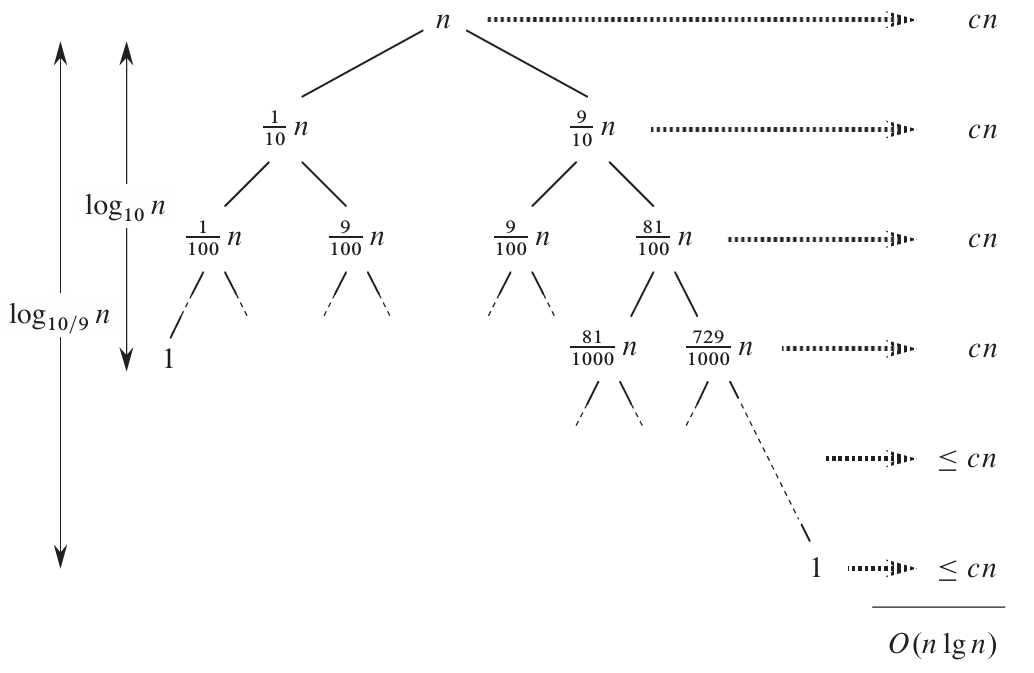
\includegraphics[scale=0.3]{convergence_avg_case.png}
    \caption{Diagrama de particiones desbalanceadas. Imagen obtenida de\cite{intro_algo}.}\label{fig:avg_case}
\end{figure}

Como se puede ver el número de niveles de recursión llegará a ser $\log_{10/9}{n}$ en la rama de la derecha, y en la rama de la izquierda será $\log_{10}{n}$.\par
Podemos simplificar estos logaritmos haciendo uso de la fórmula de cambio de base:

\begin{equation}
    \log{a} = \log{b}\cdot \log_b{a}
\end{equation}
Y posteriormente, por nomenclatura de notación Big O, podemos ignorar la constante que aparece.\par

Para cada nivel de recursión se tendrán que hacer $\approx n$ operaciones, resultando en la complejidad de: $\Theta(n\cdot \log{n})$.

Sabiendo esto es simple entender porqué es necesaria una buena técnica para escoger el pivote.
\par Una técnica muy popular y relativamente sencilla de entender el agarrar el primer, último y elemento de el medio del arreglo o partición, 
calcular su mediana y usar eso como pivote.
Esta técnica ayuda a que el quicksort pase de tener una complejidad del peor caso para arreglos ordenados al mejor caso, y también ayuda a siempre tener dos particiones de longitud distintas a cero.

\subsection{Algoritmos de ordenamiento in-place}
Quicksort es un algoritmo in-place, lo que significa que funciona haciendo intercambios sin hacer uso de estructuras de datos externas. Otros algoritmos que son in-place serían ambas versiones del Bubblesort, Insertion sort y el Selection sort.
La gran ventaja de usar este paradigma es que la complejidad espacial del algoritmo es bastante baja, $\Theta(\log{n})$ en el mejor caso y caso promedio y $O(n)$ en el peor caso.
Sin embargo, si hacemos uso de la técnica de la mediana de tres para escoger el pivote, nos aseguramos de tener una complejidad espacial logarítmica al tener los $\log{n}$ niveles.\cite{space_complexity}

\section{Metodología}
Aquí debe describir los métodos, enfoques o procedimientos utilizados en su investigación.
\subsection{Implementaciones}
\subsubsection{Quicksort}
En esta primera implementación se recreó paso a paso el pseudocódigo mencionado anteriormente en C\#, donde el pivote escogido es el elemento de la derecha del arreglo/partición.
La función principal quedó de la siguiente manera:

\begin{minted}{csharp}
void q_sort(int low, int high)
        {
            if (low < high)
            {
                int q = Partition(low, high);
                q_sort(low, q - 1);
                q_sort(q + 1, high);
            }
        }
\end{minted}

Mientras que la función partición quedó así:

\begin{minted}{csharp}
int Partition(int low, int high)
        {
            int i = low - 1;
            int pivot = Array[high];
            int temp;
            for (int j = low; j < high; j++)
            {
                NumComparisons++;
                if (Array[j] <= pivot)
                {
                    i++;
                    // swap
                    temp = Array[j];
                    Array[j] = Array[i];
                    Array[i] = temp;
                    NumSwaps++;
                }
            }

            // final swap
            temp = Array[i + 1];
            Array[i + 1] = Array[high];
            Array[high] = temp;
            NumSwaps++;

            return i + 1;
        }
\end{minted}

Añadiendo un contador de comparaciones e intercambios para cuantificar complejidad.

\subsubsection{Quicksort Optimizado}
Posterior a la implementación original del quicksort, se modificó para que el pivote sea escogido usando la mediana del primer, medio y último elemento de la partición.
Para ello se hizo una función que tiene como parámetros un arreglo y los índices inferior y superior, y su valor de retorno es el índice de la mediana de las posiciones inferior, media y superior.
\begin{minted}[breaklines=true]{csharp}
int Median_Of_3(int low, int high)
        {
            int middle = (low + high + 1) / 2;
            int x1 = Array[low];
            int x2 = Array[middle];
            int x3 = Array[high];

            if ((x2 <= x1 && x1 <= x3) || (x3 <= x1 && x1 <= x2))
                return low;
            else if ((x1 <= x2 && x2 <= x3) || (x3 <= x2 && x2 <= x1))
                return middle;
            else
                return high;
        }
\end{minted}
Teniendo esta función lista sólo hubo que añadir dos líneas antes del ciclo for en la función partición para escoger el pivote y mandarlo al final.
\begin{minted}{csharp}

            int i = low - 1;
            int pivotIndex = Median_Of_3(low, high);
            NumComparisons++;
            // swap pivot con high
            NumSwaps++;
            int temp = Array[pivotIndex];
            Array[pivotIndex] = Array[high];
            Array[high] = temp;

            int pivot = Array[high];
\end{minted}

\subsubsection{Bubblesort}
Para poder hacer una comparativa al quicksort se implementaron tanto el Bubblesort como el Flag Bubblesort, teniendo la implementación del Bubblesort así:

\begin{minted}[breaklines=true]{csharp}
void B_Sort()
{
    for (int i = 0; i < n - 1; i++)
    {
        for (int j = 0; j < n - i - 1; j++)
        {
            NumComparisons++;
            if (Array[j + 1] < Array[j])
            {
                // Swap
                int temp = Array[j + 1];
                Array[j + 1] = Array[j];
                Array[j] = temp;

                NumSwaps++;
            }
        }
    }
}
\end{minted}
Y para el Flag Bubblesort sólo se anadió el flag de intercambio:
\begin{minted}[breaklines=true]{csharp}
void FB_Sort()
        {
            for (int i = 0; i < n - 1; i++)
            {
                bool swapped = false;
                for (int j = 0; j < n - i - 1; j++)
                {
                    NumComparisons++;
                    if (Array[j + 1] < Array[j])
                    {
                        int temp = Array[j + 1];
                        Array[j + 1] = Array[j];
                        Array[j] = temp;

                        NumSwaps++;
                        swapped = true;
                    }
                }
                if (!swapped)
                {
                    break;
                }
            }
        }
\end{minted}
Ambas implementaciones tienen un contador de operaciones e intercambios para medir complejidad.

\subsubsection{Insertionsort}
Para implementarlo en C\# se hizo de la manera siguiente:
\begin{minted}[breaklines=true]{csharp}
void I_Sort()
        {
            for (int i = 1; i < n; i++)
            {
                var key = Array[i];
                int j = i - 1;
                while ( j >= 0 && Array[j] > key)
                {
                    NumComparisons++;
                    Array[j + 1] = Array[j];
                    j--;  
                    NumSwaps++;    
                }
                Array[j + 1] = key;
            }
        }
\end{minted}
añadiendo un contador de operaciones para cuantificar la complejidad.

\subsubsection{Selectionsort}
Para implementarlo en C\# se hizo de la manera siguiente:
\begin{minted}[breaklines=true]{csharp}
void S_Sort()
        {
            for (int i = 0; i < n - 1; i++)
            {
                int min = i;

                for (int j = i + 1; j < n; j++)
                {
                    NumComparisons++;
                    if (Array[j] < Array[min])
                    {
                        min = j;
                    }
                }
                NumSwaps++;
                int temp = Array[i];
                Array[i] = Array[min];
                Array[min] = temp;
            }
        }
\end{minted}
añadiendo un contador de operaciones para cuantificar la complejidad.

\subsubsection{Generador de arreglos}
Se crearon dos funciones para poder probar nuestras implementaciones con arreglos de longitud n.\par
La primera genera $n$ elementos aleatorios de la siguiente manera:

\begin{minted}{csharp}
int[] rand_n_array(int n)
        {
            int[] Array = new int[n];
            Random random = new Random(100);
            int Valor;
            for (int i = 0; i < n; i++)
            {
                Valor = random.Next(0, 2 * n);
                Array[i] = Valor;
            }
            return Array;


        }
\end{minted}

Cabe aclarar que se usa una semilla para asegurar reproducibilidad pero no es necesaria.\par
Mientras que la segunda función genera $n$ elementos ordenados de menor a mayor:

\begin{minted}{csharp}
int[] n_array(int n)
        {
            int[] Array = new int[n];
            for(int i = 0; i < n; i++)
            {
                Array[i] = i;
            }
            return Array;
        }
\end{minted}


\subsection{Experimentos}
\subsubsection{Quicksort vs Quicksort optimizado}
Primeramente se compararon ambas implementaciones de Quicksort en arreglos ordenados y aleatorios de longitudes desde 10 hasta 1000 elementos.\par
La elección de que el límite de longitud sea 1000 es para evitar el StackOverFlowException de C\# cuando la implementación no optimizada ordena arreglos ordenados.\par
Finalmente se guardaron los resultados en archivos csv para su posterior análisis.



\subsubsection{Quicksort optimizado vs demás algoritmos}
En el segundo experimento ahora se compararon las implementaciones del Quicksort optimizado, Bubblesort, Flag Bubblesort, Insertionsort y Selectionsort con arreglos tanto ordenados como desordenados.\par
Para los arreglos ordenados las longitudes de las listas estuvieron en el rango de 100 a 50,000 elementos y para los arreglos desordenados los rangos variaron desde 100 hasta 10,000. Esta decisión se tomó para evitar saturar la computadora debido a la complejidad $O(n^2)$ de los demás algoritmos.\par
Finalmente se guardaron los resultados en archivos csv para su posterior análisis.



\section{Resultados}
\subsection{Quicksort vs Quicksort optimizado}
Cuando se hace la comparación con arreglos desordenados obtenemos esta gráfica:
\begin{figure}[H]
    \centering
    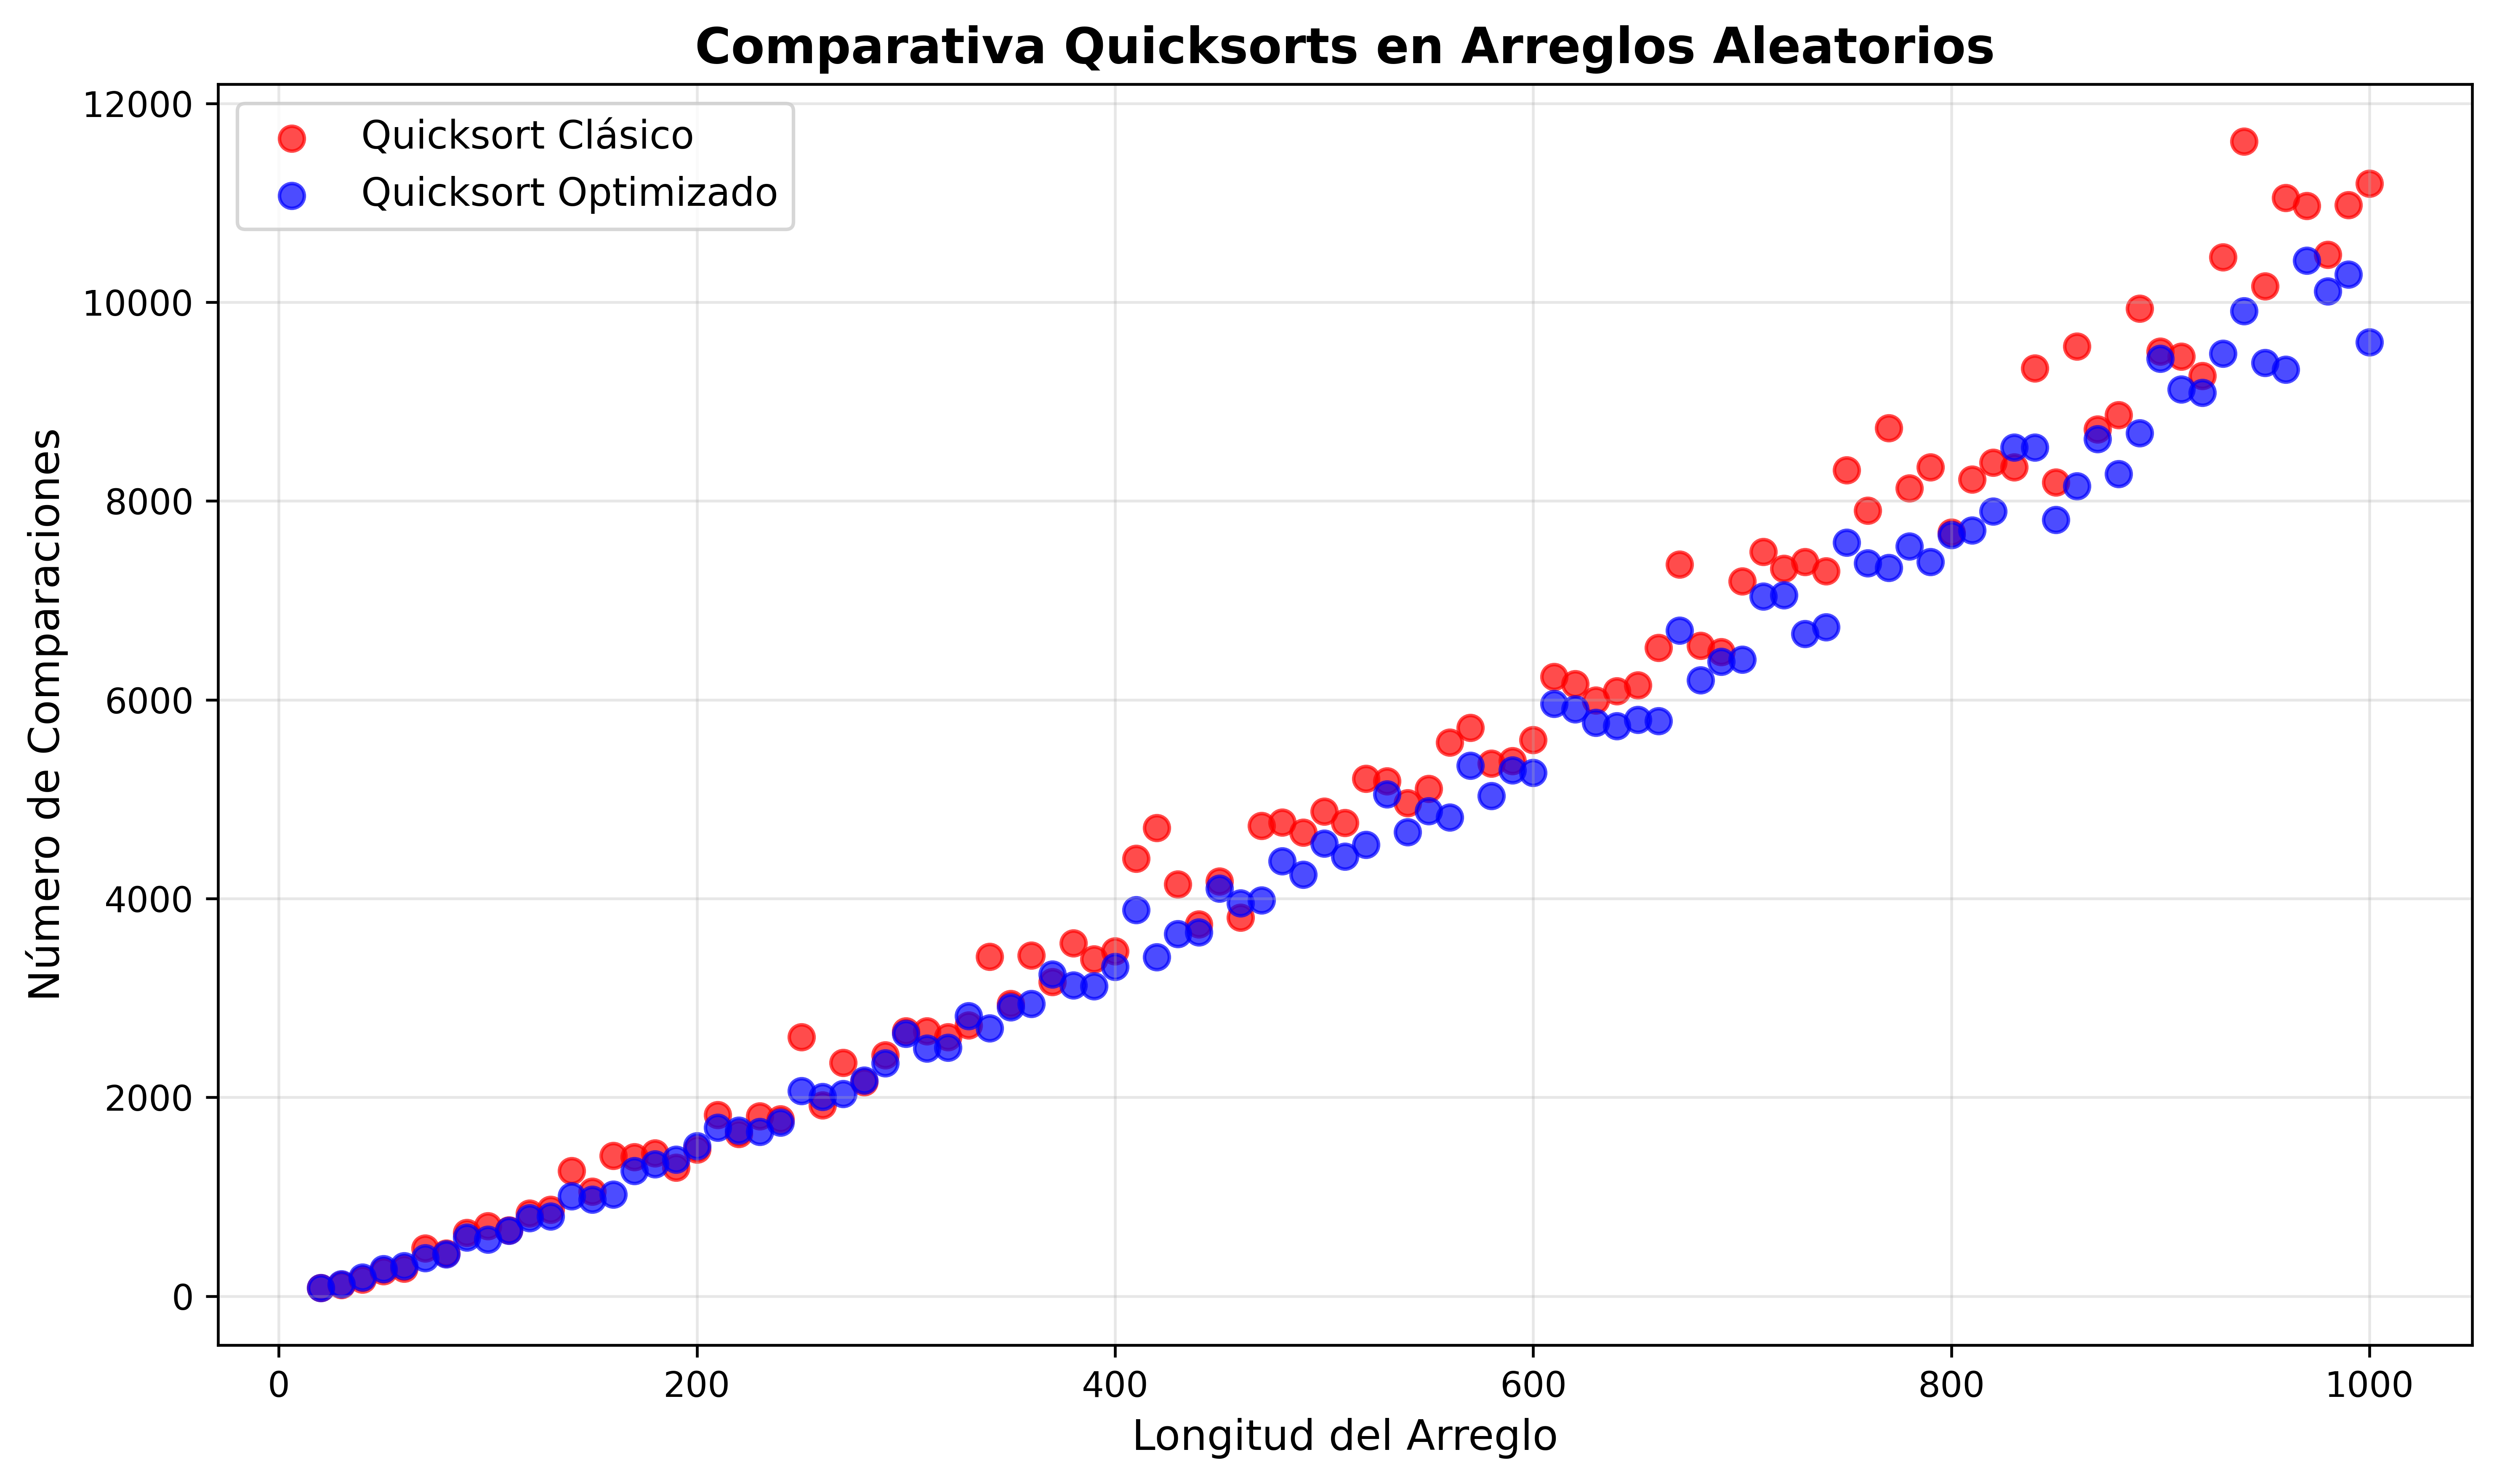
\includegraphics[scale=0.35]{../Gráficas/Exp1A.png}
    \caption{Comparativa de Quicksorts en escala lineal.}\label{fig:exp1A}
\end{figure}
Como se puede ver el quicksort optimizado es ligeramente más eficiente que el tradicional.\\
Mientras que cuando se hace la comparación con arreglos ordenados obtenemos esta otra gráfica:

\begin{figure}[H]
    \centering
    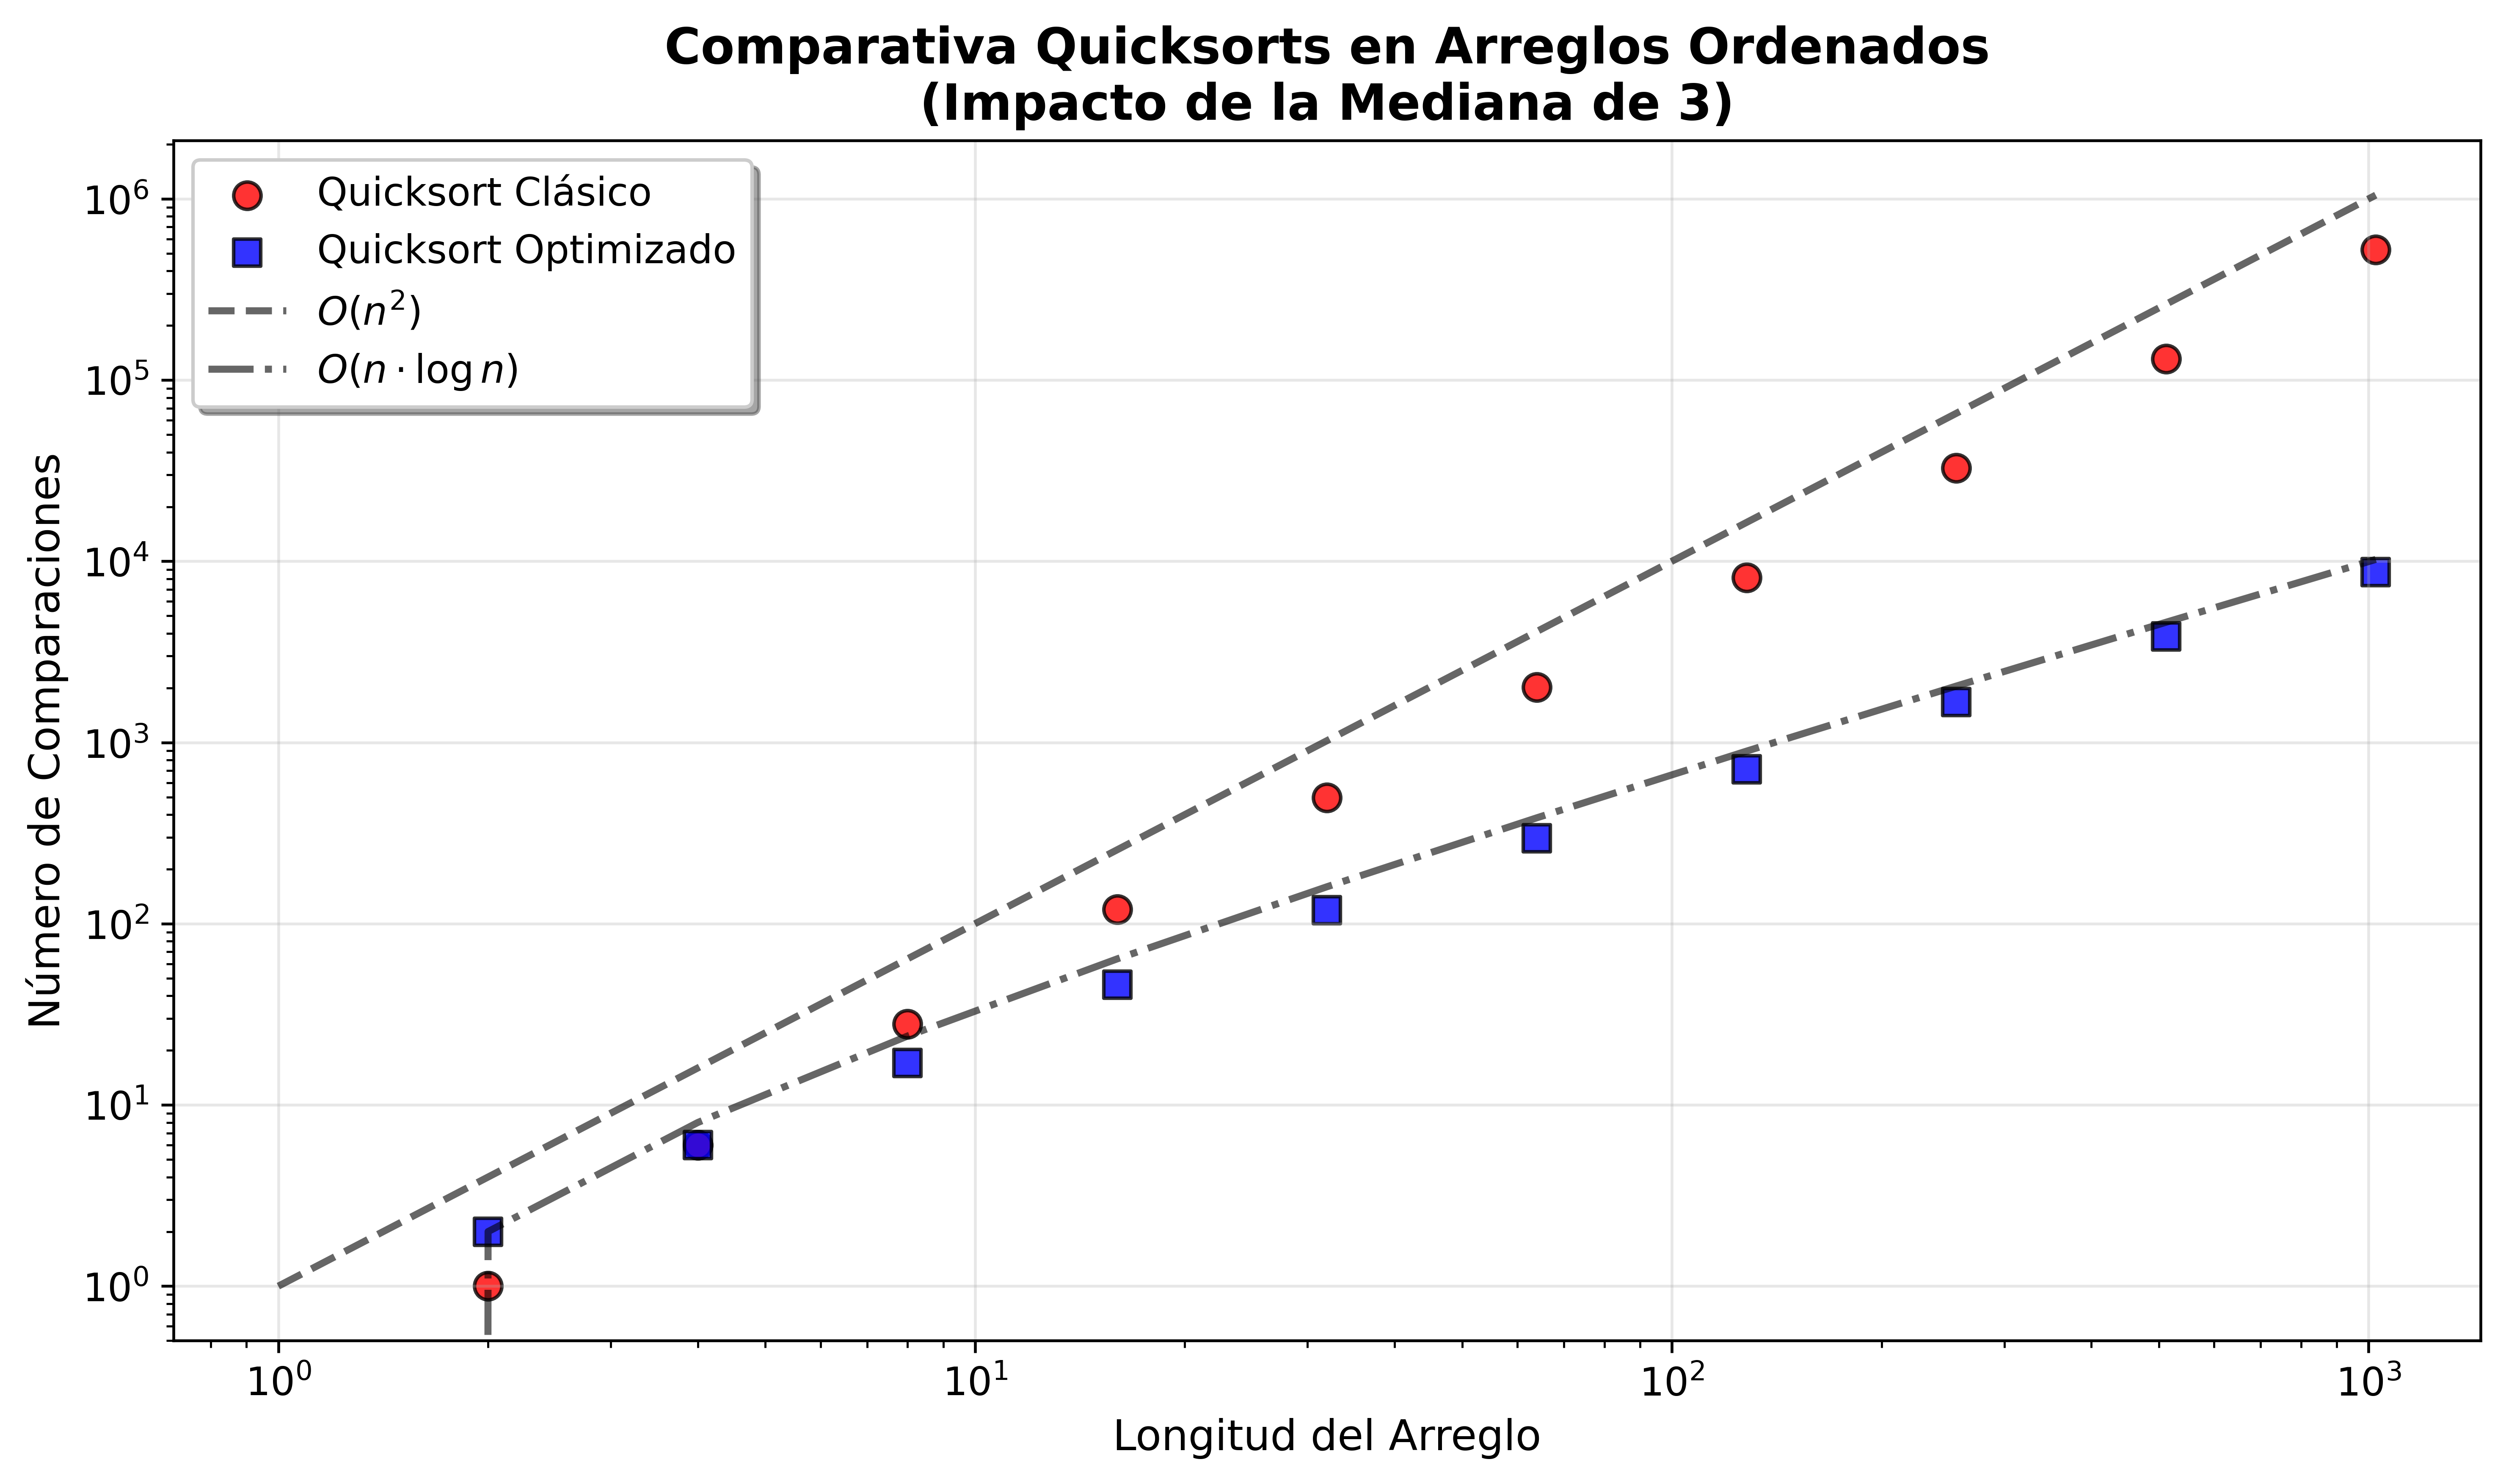
\includegraphics[scale=0.35]{../Gráficas/Exp1B.png}
    \caption{Comparativa de Quicksorts en escala logarítmica.}\label{fig:exp1B}
\end{figure}
Aquí es considerablemente mayor la diferencia, mientras que el quicksort optimizado mantiene $O(n\cdot \log{n})$ operaciones, el tradicional aumenta a $O(n^2)$ operaciones.
\subsection{Quicksort optimizado vs demás algoritmos}

Cuando se hace la comparación con arreglos desordenados obtenemos esta gráfica:

\begin{figure}[H]
    \centering
    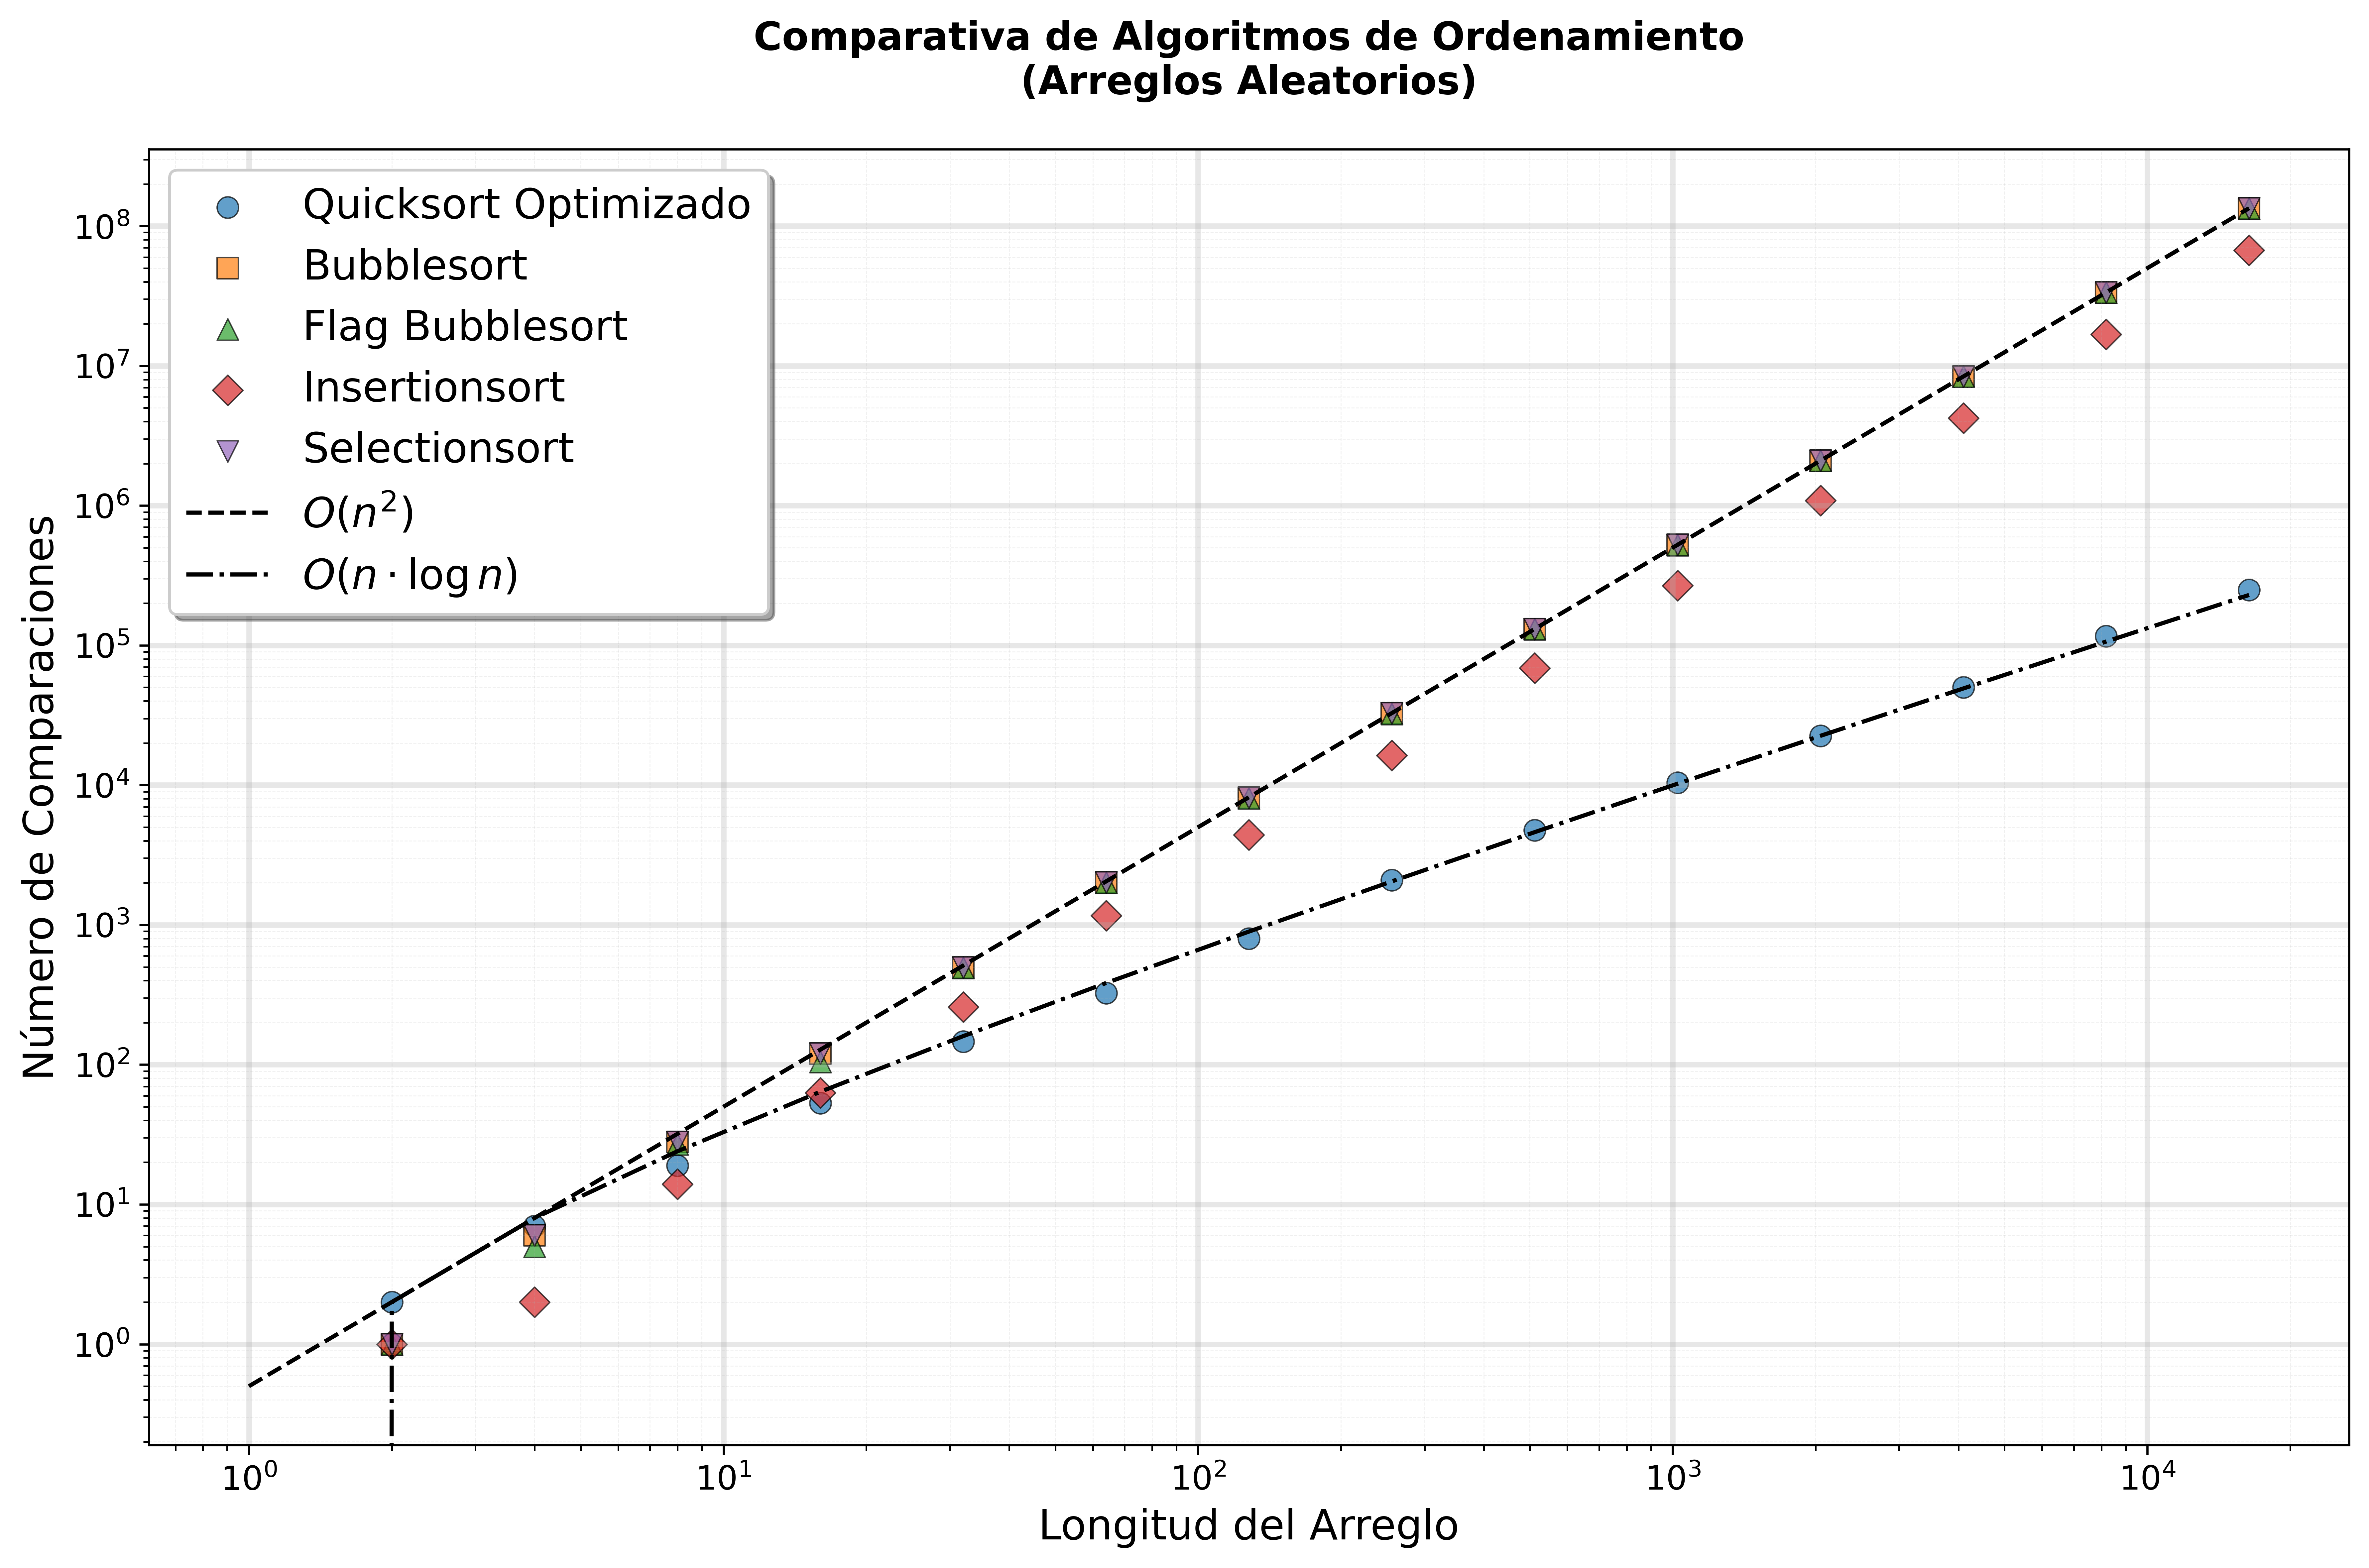
\includegraphics[scale=0.3]{../Gráficas/Exp2A.png}
    \caption{Quicksort vs demás en escala logarítmica.}\label{fig:exp2A}
\end{figure}
Aquí podemos ver como los demás algoritmos requieren de $O(n^2)$ operaciones mientras que el quicksort es constante.\\
Mientras que cuando se hace la comparación con arreglos ordenados obtenemos esta otra gráfica:

\begin{figure}[H]
    \centering
    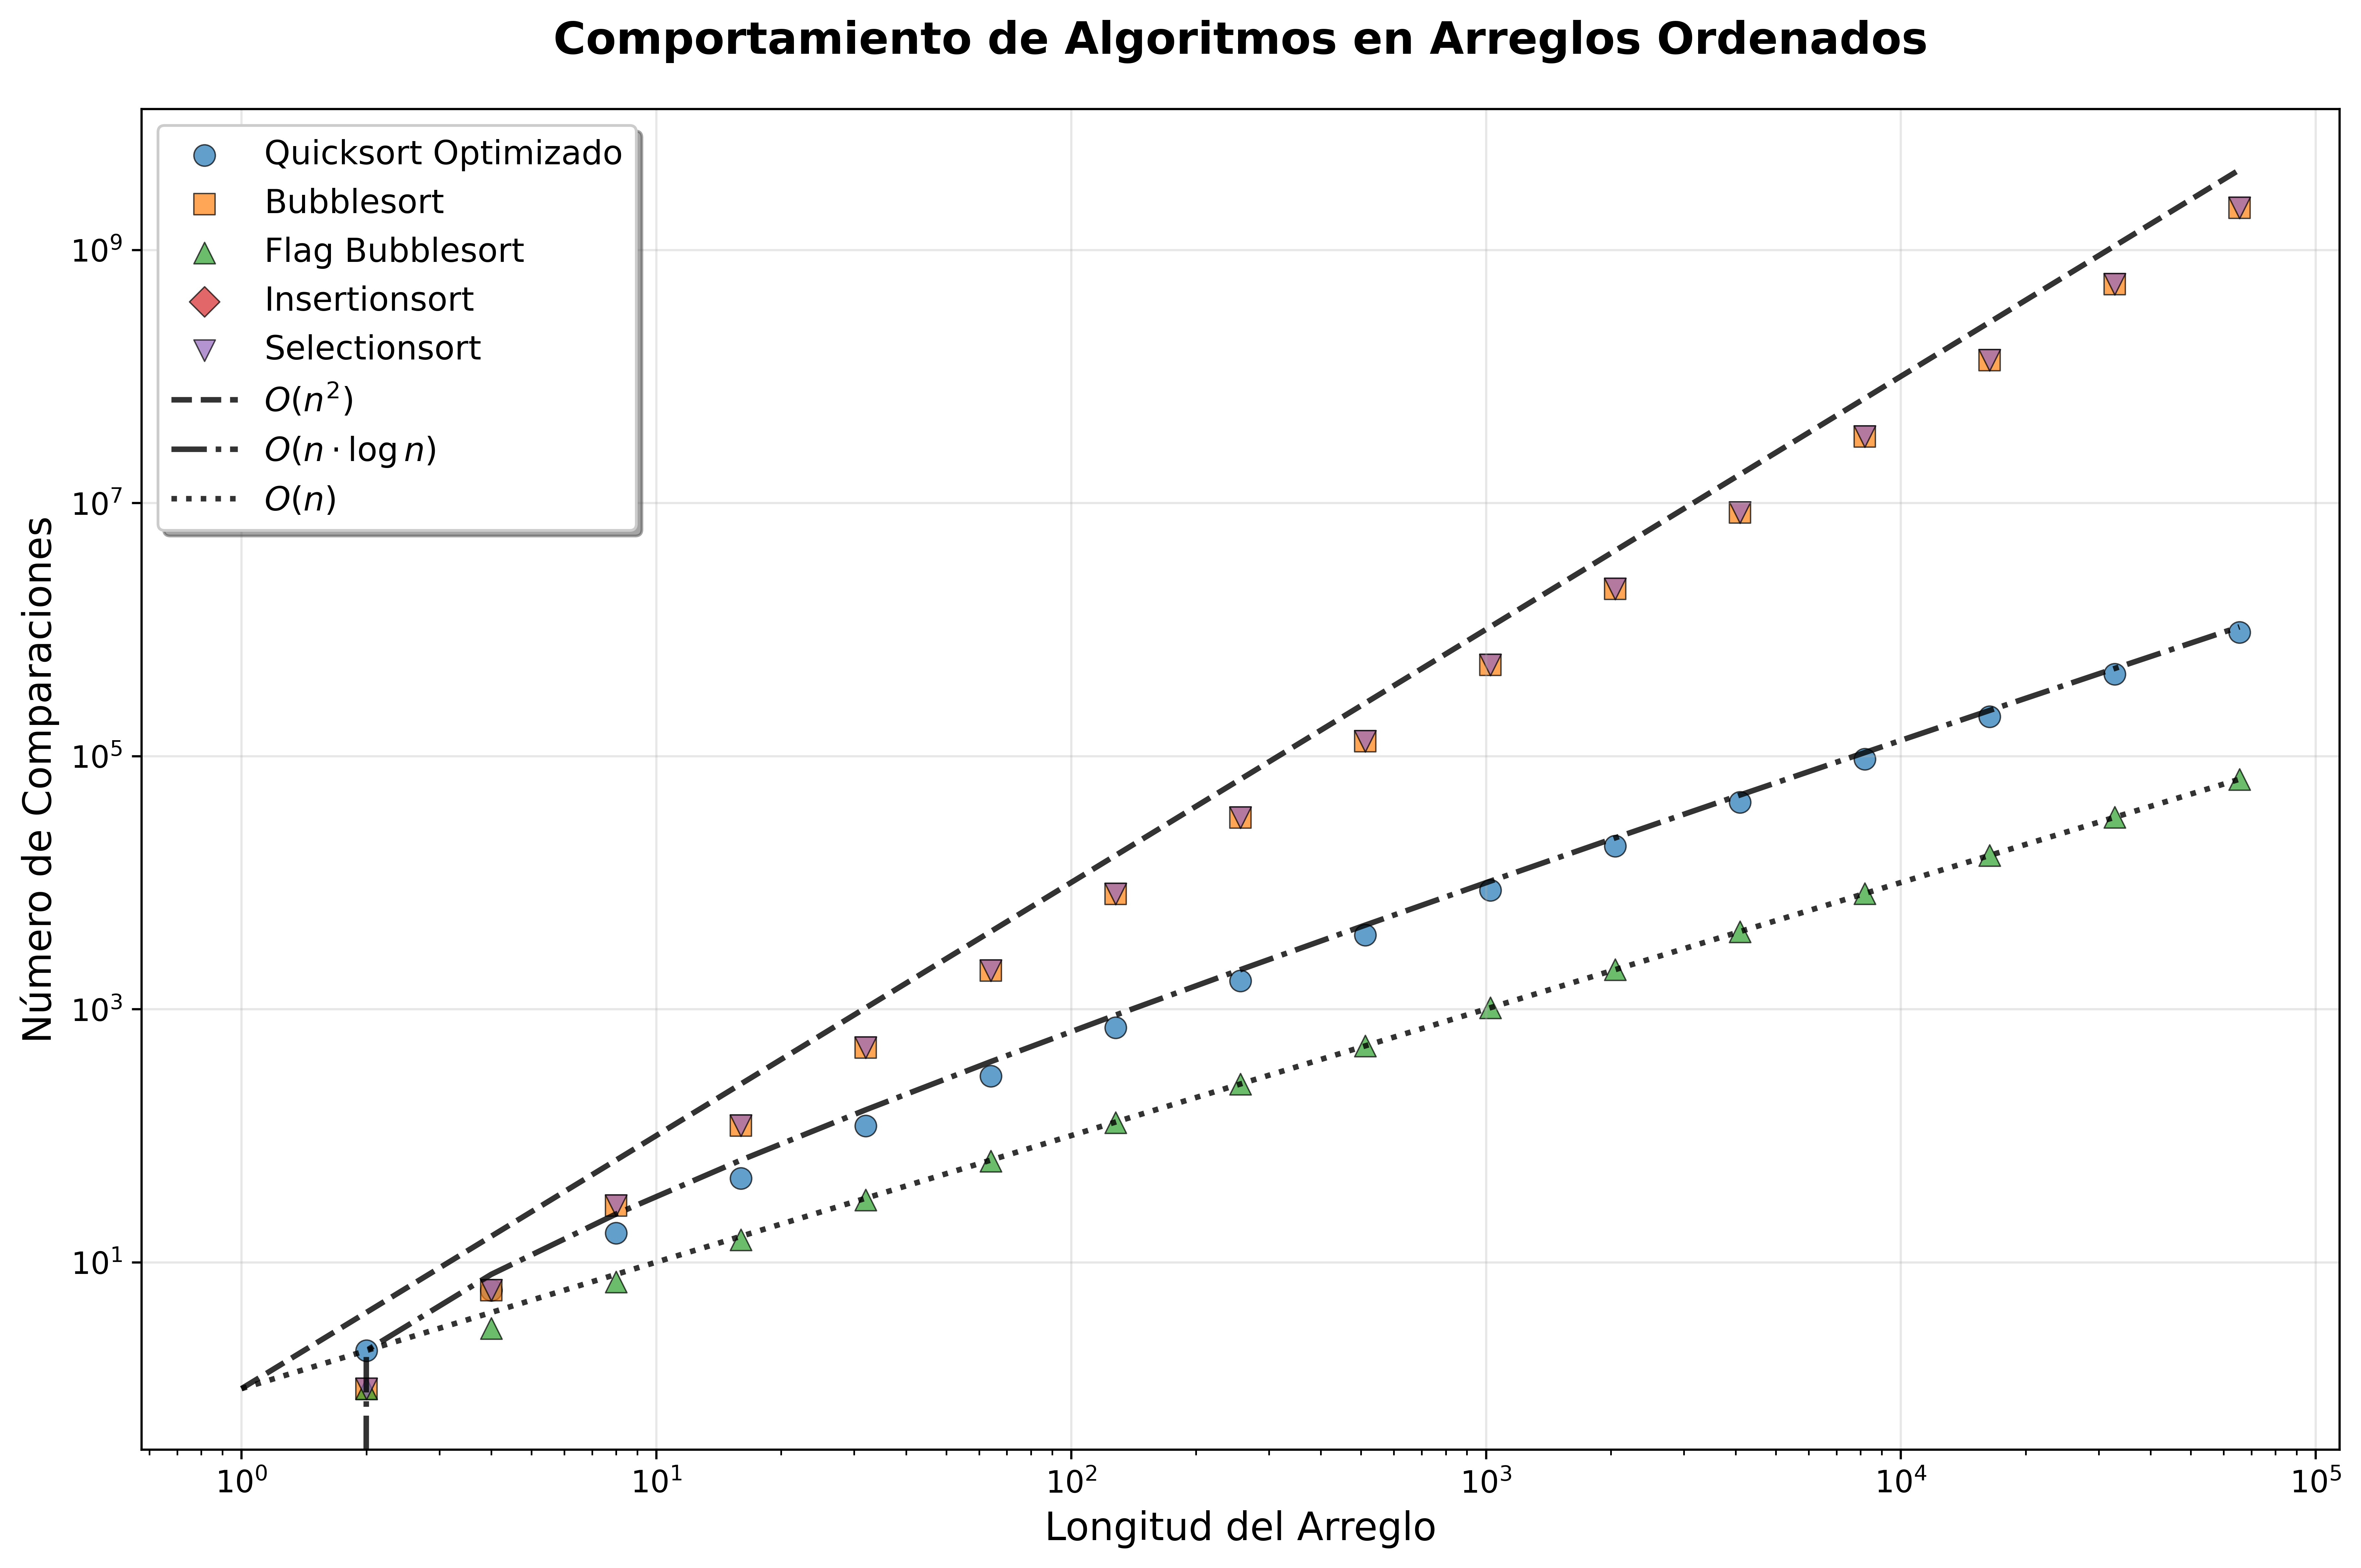
\includegraphics[scale=0.3]{../Gráficas/Exp2B.png}
    \caption{Quicksort vs demás en escala logarítmica.}\label{fig:exp2B}
\end{figure}
Aquí el Insertion Sort y el Flag BubbleSort reducen su número de operaciones a $O(n)$, mientras que los demás mantienen el número de operaciones.


\section{Conclusiones}

Después de analizar estas distintas implementaciones hay 2 puntos importantes de mencionar:

\begin{itemize}
    \item Escoger bien el pivote ayuda ligeramente en arreglos desordenados pero ayuda demasiado para arreglos ordenados y nos da una complejidad tanto temporal como espacial bastante más estable.
    \item De los algoritmos de ordenamiento in-place que se analizaron el quicksort es indiscutiblemente el ganador.
\end{itemize}

Sin embargo hay un dos preguntas que se podrían explorar a futuro:
\begin{itemize}
    \item ¿Hay alguna implementación que supere la complejidad temporal obtenida aquí revisando si el arreglo está previamente ordenado? 
    \item ¿qué otras técnicas para escoger el pivote existen y cuáles son sus respectivas complejidades?
\end{itemize}

El Quicksort es un algoritmo sumamente efectivo tanto en complejidad espacial como temporal, 
es relativamente sencillo de implementar y es bastante flexible ya que acepta distintos tipos de datos como entrada; 
haciéndolo una opción bastante sólida para diversas aplicaciones.

\bibliographystyle{IEEEtran}
\bibliography{biblios}


\appendices
\section{Repositorio}
Para ver el repositorio completo de GitHub haga click \href{https://github.com/PabloNatB/Comparativa-Quicksort}{\textbf{aquí}}.

%Algoritmos
\subsection{Implementaciones en C\#}
Para las implementaciones en C\# haga click \href{https://github.com/PabloNatB/Comparativa-Quicksort/blob/main/Qsort/Class1.cs}{\textbf{aquí}}.

%Experimentos
\subsection{Experimentos}
Para los experimentos en C\# haga click \href{https://github.com/PabloNatB/Comparativa-Quicksort/blob/main/Qsort/Program.cs}{\textbf{aquí}}.

%Resultados
\subsection{Tablas de resultados}
Para las tablas de resultados haga click \href{https://github.com/PabloNatB/Comparativa-Quicksort/tree/main/Qsort/bin/Debug/net8.0}{\textbf{aquí}}.



\end{document}

